\section{Dealing with Links}
\label{sec:links}



\subsection{Weighted Stochastic Block Model}
\label{ssec:wsbm}

\wsbm~\cite{aicher-2014-wsbm} is a generalized \emph{stochastic block
  model}~\cite[\sbm]{holland-1983-sbm,wang-1987-sbm-directed} and
predicts nonnegative integer-weight links, instead of binary-weight
links.  A block is a collection of documents which are densely
connected with each other but sparsely connected with documents in
other blocks.  \wsbm assumes that a document belongs to exactly one
block.  A link connecting two documents in blocks~$l$ and~$l'$ has a
weight generated from a Poisson distribution with parameters~$\Omega_{l,l'}$ which has a Gamma prior with parameters~$a$ and~$b$, as
Figure~\ref{fig:wsbm} shows.

\begin{figure}[t!]
  \centering
  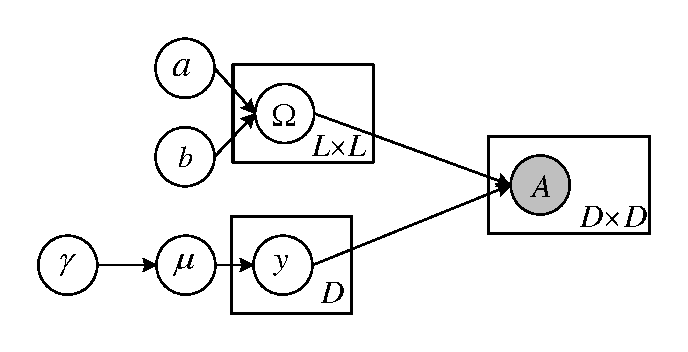
\includegraphics[width=.8\linewidth]{2016_acl_docblock/figures/wsbm.pdf}
  \caption{Weighted Stochastic Block Model}\label{fig:wsbm}
\end{figure}

The whole generative process is:\par\nobreak
\begin{small}
\begin{enumerate}[leftmargin=*,noitemsep]
\item For each pair of blocks $(l,l')\in \{1,\ldots,L\}^2$
    \begin{enumerate}
    \item Draw inter-block link rate $\Omega_{l,l'}\sim \mathrm{Gamma}(a,b)$
    \end{enumerate}
\item Draw block distribution $\bm{\mu}\sim \mathrm{Dir}(\gamma)$
\item For each document $d\in \{1,\ldots,D\}$
    \begin{enumerate}
    \item Draw block assignment $y_d\sim \mathrm{Mult}(\bm{\mu})$
    \end{enumerate}
\item For each link $(d,d') \in \{1,\ldots,D\}^2$
    \begin{enumerate}
    \item Draw link weight $A_{d,d'} \sim \mathrm{Poisson}(\Omega_{y_d,y_{d'}})$
    \end{enumerate}
\end{enumerate}
\end{small}

\wsbm is a probabilistic block detection algorithm and more robust than some
deterministic algorithms like \scc, which is vulnerable to noisy links.  For
instance, we would intuitively say Figure~\ref{fig:block} has two blocks---as
denoted by coloring---whether or not the dashed link exists.  If the dashed link
does not exist, both \wsbm and \scc can identify two blocks.  However, if the
dashed link does exist, \scc will return only one big block that contains all
nodes, while \wsbm still keeps the nodes in two reasonable blocks.

\begin{figure}[t!]
  \centering
  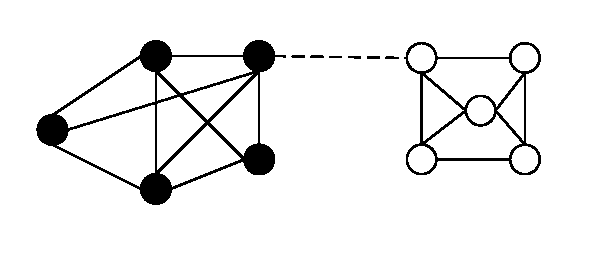
\includegraphics[width=.60\linewidth]{2016_acl_docblock/figures/block_example.pdf}
  \caption{\scc can be distracted by spurious links connecting two groups, while
    \wsbm maintains the distinction.}\label{fig:block}
\end{figure}

\subsection{Relational Topic Model}
\label{ssec:rtm}


\begin{figure}[t!]
  \centering
  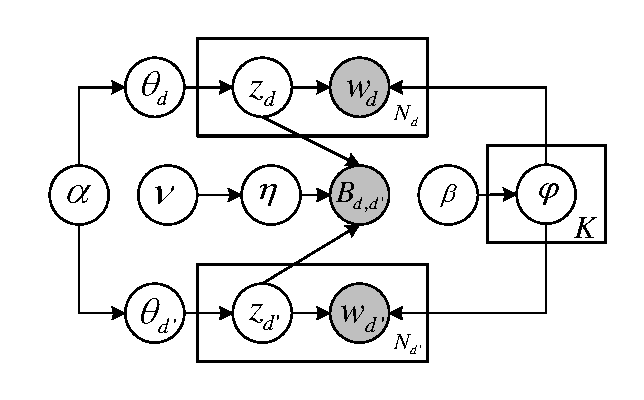
\includegraphics[width=.8\linewidth]{2016_acl_docblock/figures/rtm.pdf}
  \caption{A Two-document Segment of \rtm}\label{fig:rtm}
\end{figure}

\rtm~\cite{chang-2010-rtm} is a downstream model that generates
documents and links simultaneously (Figure~\ref{fig:rtm}).  Its
generative process is:\par\nobreak
\begin{small}
\begin{enumerate}[leftmargin=*,noitemsep]
\item For each topic $k\in \{1,\ldots,K\}$
    \begin{enumerate}
    \item Draw word distribution $\bm{\phi_k}\sim \mathrm{Dir}(\beta)$
    \item Draw topic regression parameter $\eta_k\sim \mathcal{N}(0,\nu^2)$
    \end{enumerate}
\item For each document $d\in \{1,\ldots,D\}$
    \begin{enumerate}
    \item Draw topic distribution $\bm{\theta_d}\sim \mathrm{Dir}(\alpha)$
    \item For each token $t_{d,n}$ in document $d$
        \begin{enumerate}
        \item Draw topic assignment $z_{d,n}\sim \mathrm{Mult}(\bm{\theta_d})$
        \item Draw word $w_{d,n}\sim \mathrm{Mult}(\bm{\phi_{z_{d,n}}})$
        \end{enumerate}
    \end{enumerate}
\item For each explicit link $(d,d')$
    \begin{enumerate}
    \item Draw link weight $B_{d,d'}\sim \Psi(\cdot\,|\, \bm{z_d}, \bm{z_{d'}}, \bm{\eta})$
    \end{enumerate}
\end{enumerate}
\end{small}

In the inference process, the updating of topic assignments is guided
by links so that linked documents are more likely to have similar
topic distributions.  Meanwhile, the linear regression (whose
output is fed into link probability function~$\Psi$) is updated to
maximize the network likelihood using current topic assignments.
